\documentclass[10pt]{article}
\textheight = 21cm
\textwidth = 15cm
\topmargin = -0.5cm
\oddsidemargin = 1cm

\usepackage{amsmath}
\usepackage[utf8]{inputenc}
\usepackage[spanish]{babel}
\usepackage{graphicx}
\usepackage{fancyhdr}
\usepackage{epstopdf}
\usepackage{titling}
\usepackage{fancyvrb,fancybox,calc} 
\usepackage[svgnames]{xcolor} 
\usepackage{enumerate}
\usepackage{adjustbox}
\usepackage{tabu}
\usepackage{multicol}
\usepackage{float}
\usepackage{subcaption}

\newcommand{\HRule}{\rule{\linewidth}{0.5mm}}
\DeclareGraphicsExtensions{.pdf,.png,.jpg}

\parindent=0mm

\definecolor{light-gray}{gray}{0.94}
\definecolor{textgray}{gray}{0.5}
\newenvironment{verbcode}{\VerbatimEnvironment
  \begin{Sbox} \color{textgray}\scriptsize
  \begin{minipage}{\linewidth+2\fboxsep-2\fboxrule-12pt}    
  \begin{Verbatim}
}{\end{Verbatim}  
  \end{minipage}   
  \end{Sbox} \color{black}\normalsize
  \fcolorbox{black}{light-gray}{\TheSbox} 
} 

\begin{document}
\begin{center}

\textsc{\LARGE Sistemas de Control}\\[0.2cm]
\textsc{\Large Instituto Tecnológico de Buenos Aires}\\[0.2cm]

% Title
\HRule \\[0.2cm]
{ \huge \bfseries Entrega Final \\[0.2cm] }
\HRule \\[1cm]

\begin{multicols}{2}


% Integrantes
\columnbreak
{\raggedright
\large
\emph{Alumnos/as:} \ Bautista \textsc{Estrada} \\
\hspace*{2.5cm} Facundo \textsc{Garaguso Fernandez}\\
\hspace*{2.5cm} Joaquín \textsc{Basualdo}\\
}
\end{multicols}

\vspace{0.5cm}

\begin{adjustbox}{max width=\textwidth}
\renewcommand{\arraystretch}{1.5}
  \begin{tabular}{|l|c|}
    \hline
    \ \ \ Nota Final    &              \\ \hline \hline
    \ \ \ Firma y Fecha &              \\ \hline
  \end{tabular}
\end{adjustbox}

\end{center}

\vspace{0.2cm}

\pagestyle{fancy}
\headheight=60pt
\fancyhead[L]{Sistemas de Control - ITBA - 2026}        
\fancyhead[R]{Entrega Final}

\newpage

% ============================================
%           Ejercicio 1
% ============================================
 
\section*{Ejercicio 1}
\begin{figure}[H]
    \centering
    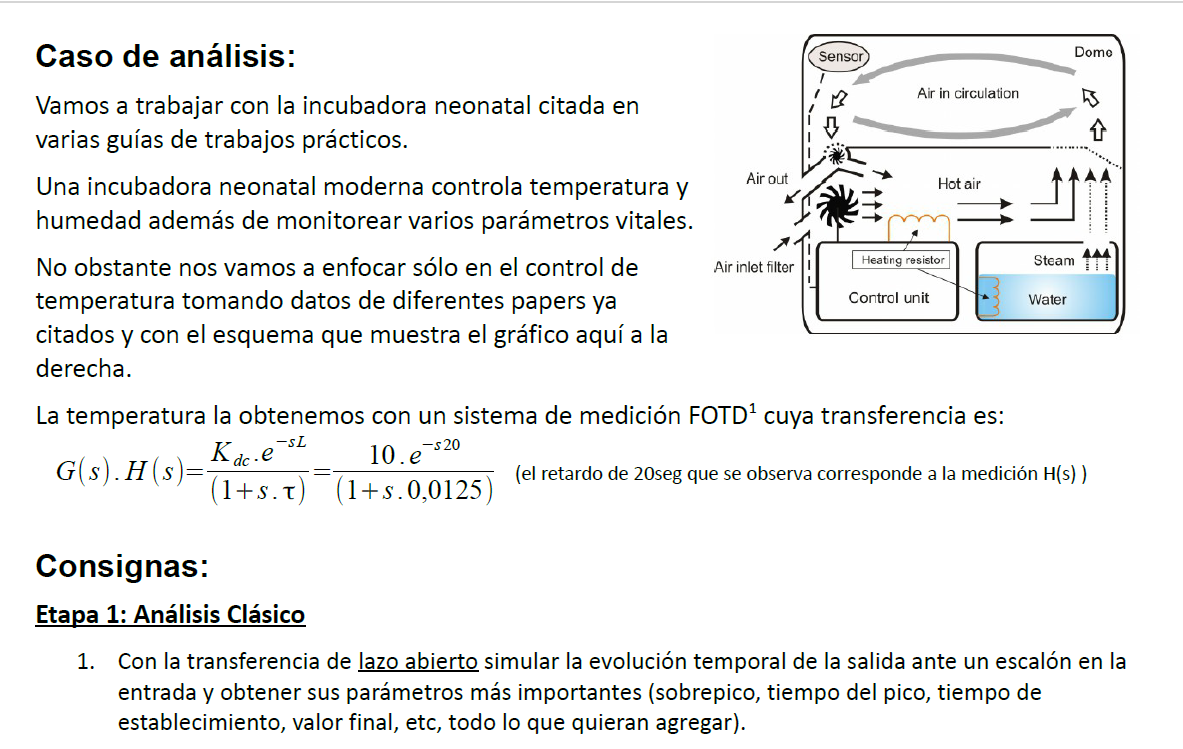
\includegraphics[width=\textwidth]{Imagenes/Ej1.png}
\end{figure}

En esta sección se analiza la respuesta temporal del sistema a lazo abierto ante
un escalón unitario en la entrada. La transferencia de lazo abierto es un modelo
de primer orden con retardo (FOTD):
\begin{equation}
  G(s)\,H(s) = \frac{K_{dc}\, e^{-sL}}{1+s\tau}
  = \frac{10\, e^{-20s}}{1+0{,}0125\,s},
\end{equation}
con ganancia $K_{dc}=10$, retardo $L=20$~s y constante de tiempo
$\tau=0{,}0125$~s.

\subsection{Aproximación del retardo por Padé}

El término $e^{-sL}$ no es un cociente de polinomios, por lo que no puede tratarse
con las herramientas del análisis clásico (lugar de raíces, criterio de Routh) ni
llevarse a variables de estado. Por este motivo se lo reemplaza por la
aproximación de Padé, que consiste en buscar un cociente de polinomios cuyo
desarrollo en serie de Taylor coincida con el de $e^{-sL}$ en la mayor cantidad
posible de términos. Para primer orden, la serie del retardo es
\begin{equation}
  e^{-sL} = 1 - Ls + \frac{L^2}{2}s^2 - \dots
\end{equation}
y proponiendo $\dfrac{1+as}{1+bs}$, al igualar los términos en $s$ y $s^2$ se
obtiene $b = L/2$ y $a=-L/2$:
\begin{equation}
  e^{-sL} \approx \frac{1-\dfrac{L}{2}s}{1+\dfrac{L}{2}s} = \frac{1-10s}{1+10s}.
\end{equation}

Esta aproximación conserva el módulo unitario del retardo en todas las
frecuencias, pero reproduce correctamente su fase solo en bajas frecuencias.
Con ella, la transferencia de lazo abierto queda
\begin{equation}
  G(s)\,H(s) \approx \frac{10\,(1-10s)}{(1+0{,}0125\,s)(1+10s)},
\end{equation}
con polos en $s=-80$ y $s=-0{,}1$, y un cero en $s=+0{,}1$. Este cero en el
semiplano derecho hace que el modelo aproximado sea de fase no mínima.

\subsection{Simulación}

Se simuló la respuesta al escalón en Python con la biblioteca
\texttt{python-control}, comparando la respuesta exacta (el escalón de primer
orden desplazado $20$~s) con las aproximaciones de Padé de órdenes 1, 2 y 3.
En las figuras siguientes se observa que todas las aproximaciones alcanzan el
mismo valor final, $y(\infty)=K_{dc}=10$, ya que Padé no modifica la ganancia en
continua. Sin embargo, durante el tiempo muerto ninguna de ellas permanece en
cero como la respuesta exacta: al no poder representar un retardo puro, una
función racional ``compensa'' con una respuesta inversa inicial. Este efecto es
un artefacto de la aproximación y no un comportamiento del sistema físico, y
resulta muy marcado en este caso porque la planta ($\tau=0{,}0125$~s) es mucho
más rápida que el rango de frecuencias en el que Padé es válido.

\end{document}